% Name: Residual block
% Description: The building block of ResNet: two weight layers learn the residual F(x), and the identity shortcut adds x back before the last ReLU.
% Tags: residual block, ResNet, skip connection, deep learning

\usetikzlibrary{arrows.meta, positioning, decorations.pathreplacing}

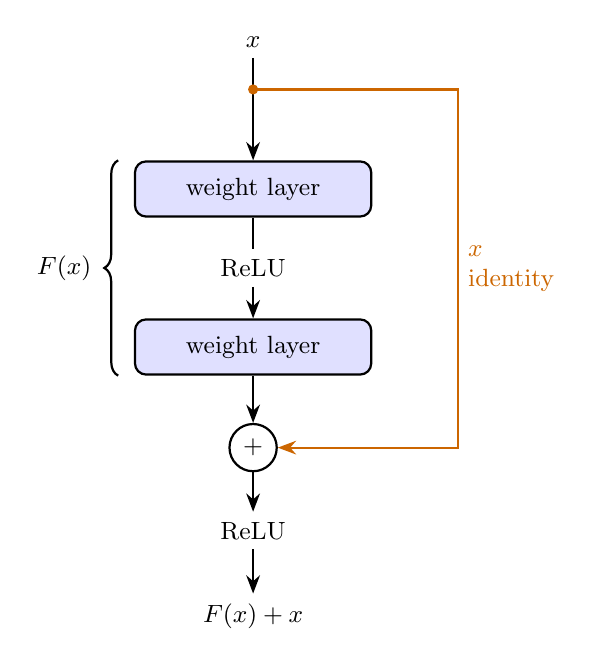
\begin{tikzpicture}[>={Stealth}, thick, node distance=6mm, every node/.style={font=\small},
    layer/.style={draw, rounded corners, fill=blue!12, minimum width=30mm, minimum height=7mm},
    sum/.style={circle, draw, fill=white, inner sep=0pt, minimum size=6mm}]
  \coordinate (in) at (0,0);
  \node[layer, below=9mm of in] (w1) {weight layer};
  \node[below=4mm of w1] (r1) {ReLU};
  \node[layer, below=4mm of r1] (w2) {weight layer};
  \node[sum, below=of w2] (add) {$+$};
  \node[below=5mm of add] (r2) {ReLU};
  \draw[->] (0,0.4) node[above] {$x$} -- (w1);
  \draw (w1) -- (r1);
  \draw[->] (r1) -- (w2);
  \draw[->] (w2) -- (add);
  \draw[->] (add) -- (r2);
  \draw[->] (r2) -- ++(0,-0.8) node[below] {$F(x) + x$};
  % The shortcut leaves above the first layer and rejoins at the sum.
  \draw[->, orange!80!black] (0,0) node[circle, fill, inner sep=1.3pt] {} -- (2.6,0) |- node[pos=0.25, right, align=left] {$x$\\identity} (add);
  \draw[decorate, decoration={brace, amplitude=5pt}] (w2.south west) ++(-2mm,0) -- ([xshift=-2mm]w1.north west) node[midway, left=6pt] {$F(x)$};
\end{tikzpicture}
